% 
% please annotate anything you need to communicate under a procentsign



 
 \begin{teaserfigure}
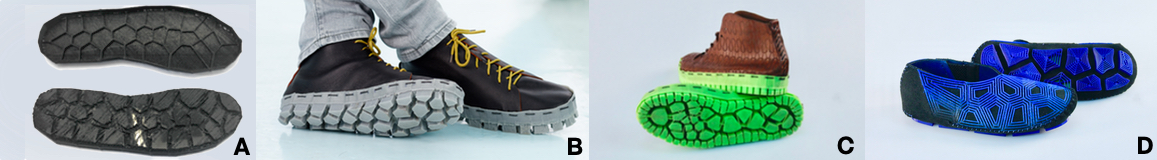
\includegraphics[width=.99\textwidth]{Header}
\caption{}
\label{fig:header}
\end{teaserfigure}

\section{Introduction}
The relationship of data and materials has long fascinated HCI and interaction design as seen in tangible bits \cite{Ishii1997}. More than a decade ago, computational composites \cite{Vallgarda2007} addressed making things with data. More recent research about the materiality of data by Dourish et al. \cite{Dourish2017} , personalization using data by Benford et. al. \cite{Benford2017}, and iterative design by researchers at Autodesk \cite{Nourbakhsh2016} opens up new design spaces. Additionally, Vallg\aa rda et al \cite{Vallgarda2015} have shown the importance of time in design. Thinking about time and access to complex data allows to design the behavior of things thanks to advances in metamaterials \cite{Ion2018a}, material programming \cite{Vallgarda2016}, and data science. 

Many makers, designers and design researchers have adopted these materials in a form of hybrid craft that enables new kinds of personalized objects. This can be seen in the work of Benford et al, \cite{Benford2018} Devendorf and Ryokai \cite{Devendorf2015}, Efrat et al. \cite{Efrat2016} and Magrisso et al. \cite{Magrisso2018}. At the same time, we have seen our understanding of design change in the form of research products \cite{Odom2016}, design with time \cite{Odom2018} and data-enabled design  \cite{Bogers2016a}. We need to only look around to find objects creating data about our everyday life. Moreover, digital fabrication allows new opportunities for encoding data into materials. When placed in the context of iterative personalization, things rarely dreamed of outside bespoke tailoring or science fiction become possible. In order to deeply understand these new data and material relationships we chose shoes as our context of application and research through design as our research method.

There are three reasons why shoes are a good artifact to research iterative personalization: 1) human movement is rich with data \cite{Shanthikumar2010}, 2) there is a long history of bespoke shoe personalization \cite{Ball1935}\cite{Greene2018}, and 3) most people go through many shoes in a year \cite{Vertommen2011}. Additionally, many companies including Nike, Adidas, Feetz, Ecco, Under Armor, and United Nude are exploring data driven, digitally fabricated, personalized shoes. Their (and our) current challenge is to create a system where the shoes themselves create a data trail for the next pair of shoes. To tackle this challenge, we used a research through design method. We created our own bespoke shoes by developing tools and techniques that explore data/material relations in personalized shoe design. We used a theoretical model of Ultra Personalized Products and Services (UPPS) \cite{stolwijk2018going} to build on our understanding of iterative personalization. Four projects based on the phases of UPPS model, fig. \ref{fig:UPPSmodel}, allowed us to complete a loop where shoes are not only personalized by parameters, but also generate data for the next pair of shoes (fig 1D). Focus was given to encoding materials (creating shoes for the form, movements and behavior of the foot) and encoding data (recording form and pressure over time) to generate increasingly personalized shoe iterations. 

\begin{figure}
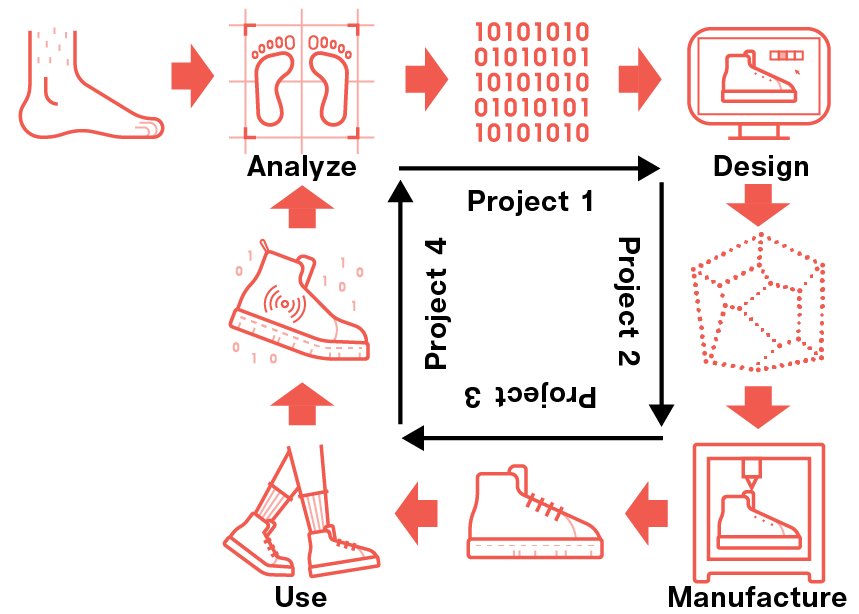
\includegraphics[width=.5\textwidth]{UPPSmodel}
\caption{Adaptation of the Ultra Personalized Products and Services (UPPS) system model describing the loop of iterative personalization for shoe design.}
\label{fig:UPPSmodel}
\end{figure}

We clearly did not have the resources to invest in an entire shoemaking factory. Instead, we digitally fabricated a series of shoes using 3D printing, laser cutting, digital embroidery and hand construction. This hybrid craft \cite{Devendorf2015} process was inspired by bespoke shoemaking (bespoke is considered one step above tailored, comparable to `engineered to order'). Being fitted for a pair of bespoke shoes goes beyond the length and width of a foot. The artisan shoemaker looks at current shoes for traces of use. They observe how a person walks for signs of behavior. They feel the foot to understand the bones, ligaments and soft tissue of the foot. They converse about pain and lack of sensation. Detailed notes and past experience lead to tiny adjustments of the last (base form of the foot to create a personalized shoe) that adjusts the shoe to the movement and behavior of the wearer. Only then an artisan shoemaker shoe is made using a signature style. 

This research unpacks the first-hand challenges and learnings we experienced in making the first full shoes that show the potential of ultra-personalized research products, and invites design researchers to join us in encoding materials and data for iterative personalization.

\section{BACKGROUND \& RELATED WORK }

More than a decade has passed since Vallg\aa rda and Redstr\"om \cite{Vallgarda2007} showed the possibility of computational composites, expanding on the work on ``Computational Things'' by Halln\"as and Redstr\"om \cite{Hallnas2002}. Examples in the past decade such as ``Spyn'' \cite{Rosner2010}, hybrid craft \cite{Zoran2015}, wearing screens \cite{Devendorf2016}, personal fabrication \cite{Baudisch2017}, and metamaterials \cite{Ion2016} help to demonstrate the potential of crafting using hybrid data and material in design. 

There is a significant interest in materials that can be digitally fabricated with specific behavior. The arrival of flexible materials in desktop 3D printing (ie. TPE \& TPU) has changed how we look at the infill (inside) structures of 3D printing as in ``The Design Space of 3D Printable Interactivity'' \cite{Ballagas2018} or ``Design and fabrication of materials with desired deformation behavior'' \cite{Bickel2010}. These materials geometries have been used to make shape changing shoe treads \cite{Ion2018}. Moreover, Ion et al. have shown the aesthetic properties of these materials in ``Metamaterial Textures'' \cite{Ion2018a}, the possibility of behavior in ``Metamaterial Mechanisms'' \cite{Ion2016} and computation in ``Digital Mechanical Metamaterials'' \cite{Ion2017}. 

\begin{figure*}[htb]
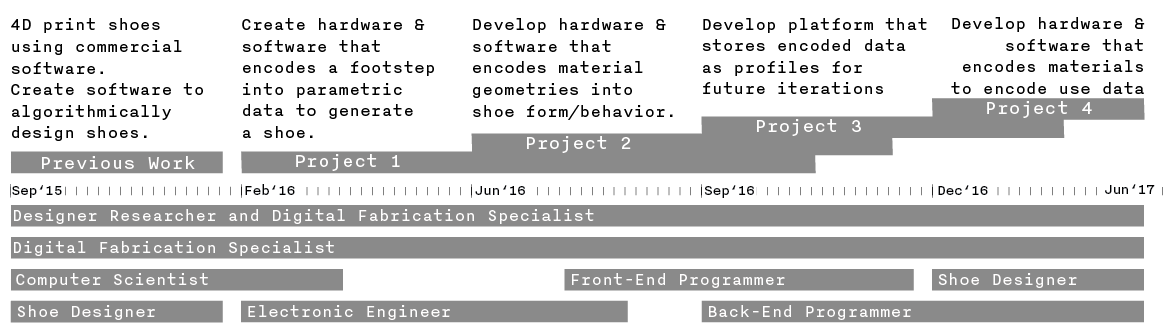
\includegraphics[width=.9\textwidth]{Timeline}
\caption{Timeline of the four projects and team members needed to complete a loop of iterative personaliztion.  }
\label{fig:timeline}
\end{figure*}

Dourish has shown data to be a material \cite{Dourish2017}. Researchers at Autodesk used data from EKG scans of a car driver to generate several iterations of a car chassis \cite{Nourbakhsh2016}. This form of iterative design created several objects from a single analysis session. This is not the only case, we see other examples of data being used as a material for design in data enabled baby bottles \cite{Bogers2016}, personalized greeting cards \cite{Benford2017} and facial makeup \cite{kao2016duoskin}. Moreover, engineering has approached the collection of data as a twinning process where the physical object and it's digital twin are mirrored \cite{Tao2018}. Many HCI shoe projects have also shown ways to generate data from shoes: ``Energy scavenging with shoe-mounted piezoelectrics'' \cite{Shenck2001} creates not only electricity but data about when it was created. ``Shoe me the way'' \cite{Schirmer2015} show the shoe as a computer and output device. ``The development of methods and procedures to determine the dynamic and functional properties of sports shoes'' \cite{Vertommen2011} describes how to record data from feet inside of shoes.  


Our research built upon the possibilities of materials and data but is situated in the following work: ``Being the Machine'' \cite{Devendorf2015}. Devendorf and Ryokai have shown the value of hybrid craft, and through their examples present a form of bespoke personalization between the maker and the machine. We used the idea of hybrid craft to join computational materials with data, resulting in the programming of an object's form, aesthetic and/or behavior for iterative personalization \cite{nachtigall2018towards}. We created fully functional shoes that create data through actual use as a research product. ``Research Prototypes to Research Products'' \cite{Odom2016} highlights the everyday experience of an object and how it can record data when constructed to have the qualities of an object in use. Finally, an ultra-personalized products and services \cite{Bhomer2016} point of view, helped us to open how HCI looks at the object, and also consider the services and systems associated with that object over a lifetime. 

\section{Research Methodology}



We engaged in this research from a Research through Design (RtD) perspective as a way of creating ``conceptually rich artifacts'' \cite{Gaver2012a}. We emphasized the material and data relationships of our designs, especially how to encode data and materials. To share our understanding of `encoding' we use a methodology inspired by ``Tangible Products'' \cite{Djajadiningrat2004} to describe the design process. The method illustrates the evolution between projects by describing each ones challenges and developing learnings that connect with the next one. Descriptions are important because they unravel the complexity of a design project and unlock the perceptions and understanding of the designer. Recent design research including ``Living In A Prototype'' \cite{Desjardins2016}, ``Productive Frictions'' \cite{Wakkary2016}, and ``Can I Wear This?'' \cite{mackey2017can} use autoethnographic techniques that include first person descriptions and observations of the context and the design itself, as described in ``Designing for, with or within'' \cite{Tomico2012}. Moreover, we see this as a form of annotated portfolio like ``The Tuning of Materials'' \cite{Karana2016}, ``Attention to detail'' \cite{Jarvis2012} and ``Annotated portfolios'' \cite{Gaver2012}.

Our methodology was informed by research products \cite{Odom2016}. Research products are high quality artifacts used as research tools that can be deployed in a natural setting. Research products hold four interdependent qualities; inquiry-driven, finish, fit, and independent \cite{Odom2016}. Our research products took the form of everyday shoes. It is like a product that is often personalized and can be created in a small digital fabrication setting such as a fab lab. Testing a full system of encoding data/materials for iterative ultra-personalized shoes could easily require an industrial process and assembly line. Yet hybrid craft and a research product methodology allowed us to synthetically engage with a system much like a bespoke shoemaker, instead of a large corporate producer.
Several personalization models could have been used for engaging in this research. ``Digital Footprint'' \cite{Benford2015} describes data enabled personalization based upon the Design, Manufacture and Use of an object. Models like ``Plantar Foot pressure to estimate foot behavior'' \cite{Hagman2005} concentrate on the analysis of the footstep. It was important for the loop of iterative personalization that the use and making phases were equally represented to account for a research product. We needed more space for analysis alongside design, manufacture, and use leading us to the theoretical model of Ultra Personalized Products and Services \cite{stolwijk2018going}. UPPS gave equal balance to the four phases and we adapted it to shoes in a system of personalization as seen in fig 2. 

Over two years, four projects were cumulatively undertaken at the Wearable Senses Lab of the Eindhoven University of Eindhoven in order to close the loop of iterative personalization. Many tools, techniques, and materials in the process were created as part of the bespoke shoemaking experience including: making/modifying 3D printers, creating pressure scanners, hacking filament sensors and creating a web architecture. We even tried to make our own filament but failed as flexible materials require large scale infrastructure. Each project required bringing together experts to help develop new machines, new software and integrate it together as shown in fig 3.

We hope that the challenges uncovered and learnings developed during these 4 projects will help to spark a deeper understanding in how iterative ultra-personalization could become an everyday reality. Do we need to return to a reality of bespoke shoemaking, or could technology, scaffold together with craft, produce a new system of designing and producing shoes?

\section{Analyzing the Four Projects Encoding Data and Materials}

\begin{figure*}
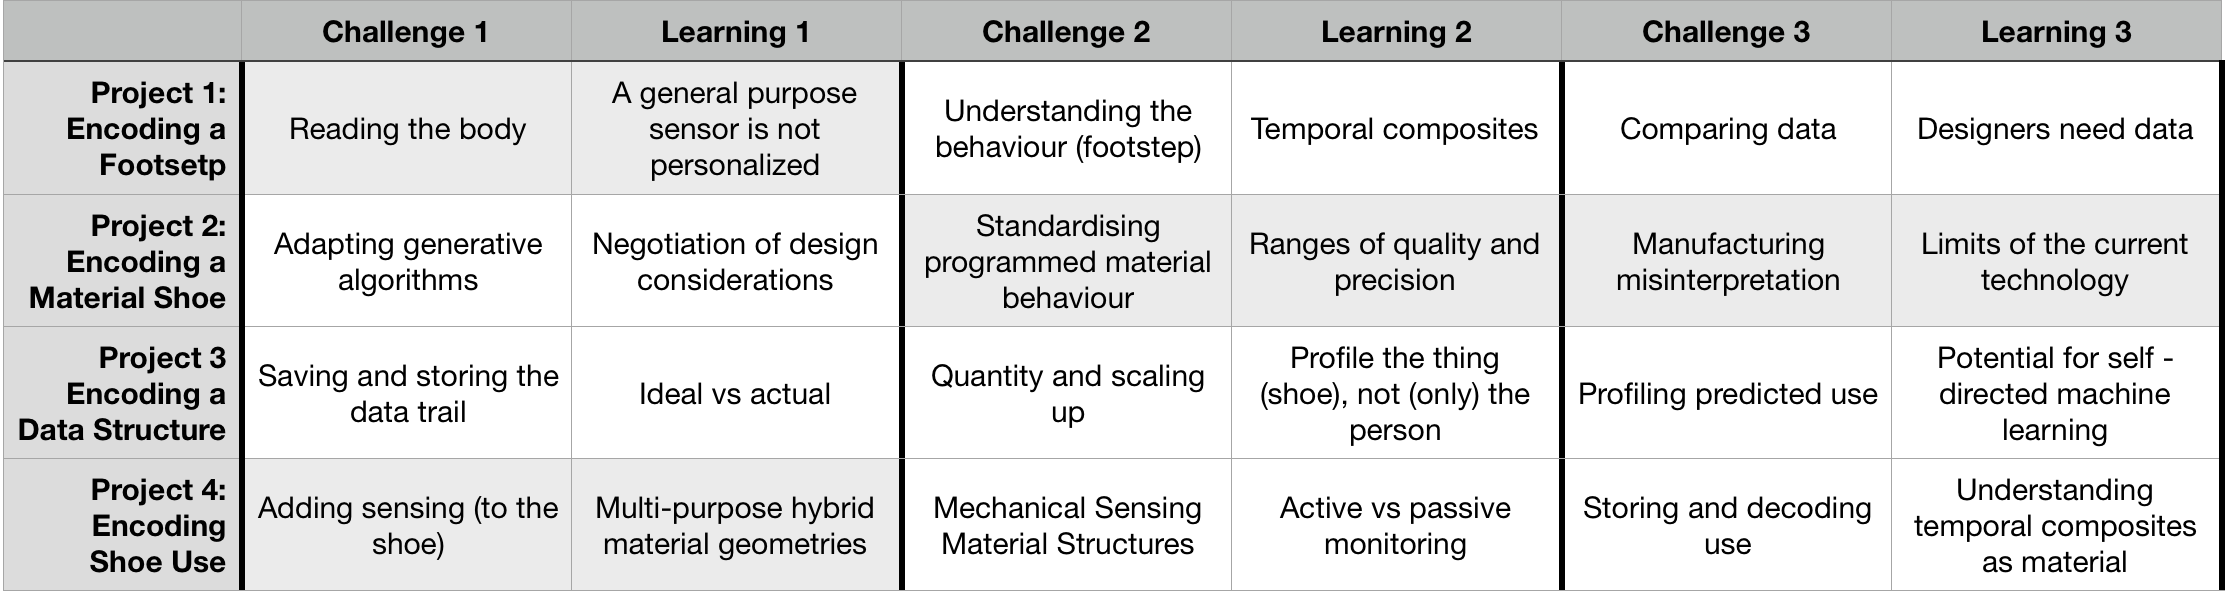
\includegraphics[width=.999\textwidth]{Table}
\captionof{table}[ChallengesLearnings]{A summary of the challenges and learnings developed over four RtD projects encoding data and materials for iterative personalization.}
\label{fig:ChallengesLearnings}
\end{figure*}

From the four projects carried out we formed an understanding of the complex system of encoding data and encoding materials that were needed to close the loop of iterative personalization. In order to make the knowledge gathered understandable and transferable, the main highlights are summarized as challenges and learnings in table 1.

Each project was built on the previous one to result in a full loop of iterative personalization. (The projects were actually iterations building upon each other, but we refer to them as `projects' to avoid confusion with ``iterative personalizaion''.)  Project 1 developed a 4D foot scanner to encode a footstep into parameters related to size and flexibility. Project 2 took the footstep parameters and negotiated them with the design considerations from bespoke shoemaking. Project 3 moved all of the software to the web to encode the data obtained over time, thus allowing the creation of data trails for one or multiple shoes. Nonetheless, it required significant software rewrites. Project 4 redesigned the shoe to encode use data for future shoes. What follows is a detailed description of how the challenges and learnings developed in each project.

\subsection{Project 1: Encoding a Footstep as Data}

The aim of project 1 was to encode a footstep as analysis data. We considered using commercially scanners like those of RS Scan which dynamically analyze footstep data \cite{Franklyn-Miller2014}, but fabricated our own as a hybrid craft project. Making our own allowed us to see the idiosyncrasies of each footstep and experience the encoding of data from scanning first hand. Commercial solutions abstract the raw data from the sensors and it was important that we experience that raw data and make our own visualization.  
Consulting with a podiatrist, the team used a digital embroidery machine to create an 8 x 16 matrix of capacitive sensors using a Cypress CY8CKIT-050 5LP to read the data at 20hz per second. The software was written in Octave in order to allow calibration and visualization in real time. Beyond the difficulties of a reliable calibration of capacitive sensing, a number of important challenges and learnings arose as we deployed the sensor at a public design exhibition and scanned over 400 feet (see figure 3). We wanted to analyze many foot sizes, from children to adults. We included children because of the public exhibition setting but they were not part of our target group because their rapid growth is a particularly difficult case.


\subsubsection{Challenge 1: Reading the body}

Determining the precision of the scanner to be suitable for general use was difficult. People have very different kinds of feet. Multiple outliers such as high arches, long toes and very thin feet were misinterpreted by our scanning software. Many of them needed special attention in the software to encode the footstep into a digital representation.  Some of them, the ones that could not be solved by software, needed sensors with different pressure ranges in specific areas of the foot. However, adjusting for one foot would make another less precise.  
After testing a series of samples, we decided on a spacing of 14 cm over 8 vertical capacitive TX lines and 1.8 cm over 16 horizontal capacitive RX lines. This was a negotiation between size and accuracy. We faced the same precision issues in relation to weight as we expected users weighing from 20kg to 130kg. The way the capacitive sensor worked was by measuring how far the foot sank into the sensor pad.  We tested industrial spacer fabrics and ended up laser cutting holes in a grid pattern for better compression under different weights. This was important as the four smaller toes of the foot apply relatively little pressure and they need to be measured.  The outcome was an image of the foot's pressure where we could even see 4mm 3D of the curve of the foot. 


\subsubsection{Learning 1: A general purpose sensor is not personalized}

The level of imprecision often seen in current scanning systems seems to be dictated by the need to make the scanner work for the general public. Personalized sensors would allow for the encoding of data to be more precise for each user. A system of iterative personalization must accept that the first iteration can only achieve a level of personalization dictated by the general purpose sensor. Fixing a problem in the sensor could only be taken to a certain precision before it would cause problems to other users. We learned to accept that the level of precision available from the general sensor could work as a starting point but more precise sensing means would be needed after each personalized iteration of the shoe. The solution would be to personalize the sensor too.

\subsubsection{Challenge 2 Understanding the behavior \(footstep\)}

Mass customization in shoes looked for ways to offer users control over color, shape and size \cite{Piller2012}. Programming materials with digital fabrication allowed us to create something far more nuanced in terms of behavior. Different areas of the foot apply pressure differently over multiple footsteps. For example, the heel, talon and big toe at times support the whole weight of the body. The smaller toes and arch rarely support significant weight. The second challenge was dealing with a footstep over time. We needed to shift the weight from the heel to the toe to understand the pressure of the foot over the footstep multiple times. Commercial systems often use a pad that can record three footsteps and a technician selects the ``best'' step. We had to adapt our software to record the size and pressure over that footstep. Dealing with static shape was already difficult, but movement was far more complex. Designing for human locomotion is complicated as many researchers have noted \cite{Lindqvist2014}\cite{Lindqvist2015}\cite{Bickel2010}.  

\subsubsection{Learning 2 Temporal composite}

We learned that it was important to deal with time and design based on movement, not just a single static moment. Instead having the data of someone standing on the sensor, the data needed was a ``temporal composite'' \cite{Koegel1992} of the footstep. Constructing this temporal composite was prone to errors as many people walk differently. The encoded data would serve as the parameters to generate the size, shape, flexibility and density of the shoe, making each shoe personal to the footstep. To do this we looked at the areas of the foot that generated each tread cell on the bottom of the shoe. The maximum impact value was translated to a density parameter for the tread and comfort in the insole. The change in pressure was used to create a flexibility parameter. 

\begin{figure}
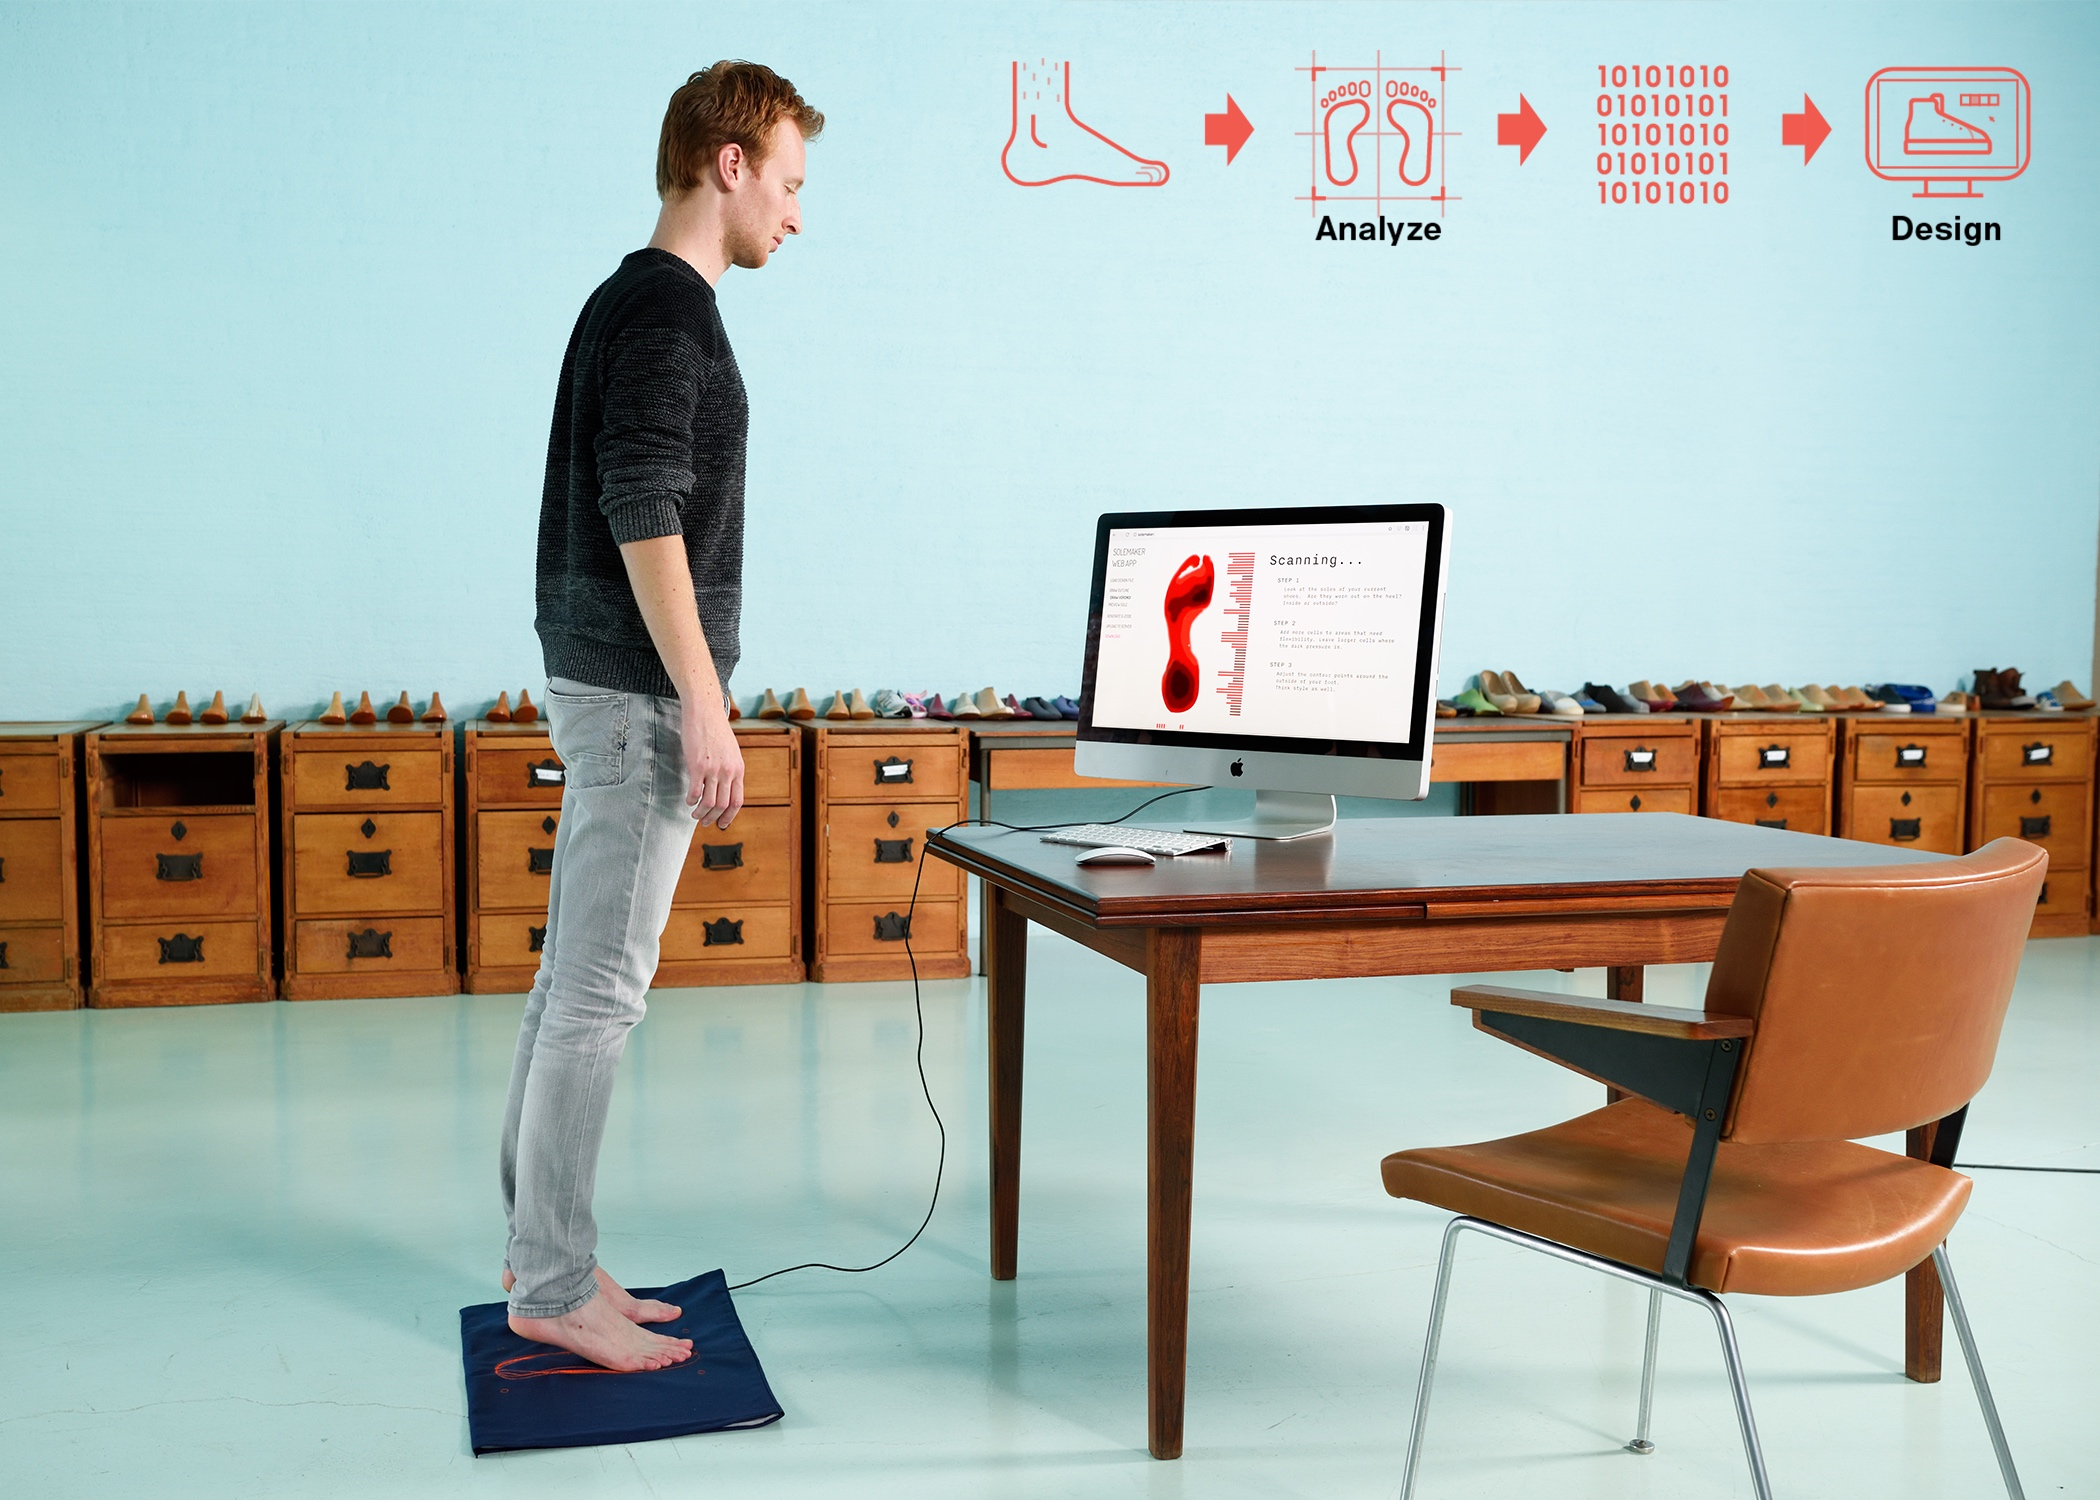
\includegraphics[width=.5\textwidth]{SoleScan}
\caption{The SoleScan pressure pad and software recorded footstep size and pressure. Photo by Bart van Overbeeke}
\label{fig:Project1}
\end{figure}

\subsubsection{Challenge 3 Comparing data}

While looking at the over 400 encoded foot scans, commonalities and specific differences emerged which are key to iterative personalization. When we scanned our own feet, we could see a difference between a morning scan and an evening scan. We consulted a podiatrist who explained us that the foot expands during the day with the pressure of the body. We found other commonalities such as the curvature of the side of the foot was softer in older than in younger people. Older people lose soft tissue with use and the feet become squarer. If we could slow the scan down (not as easy as it may seem) we would see the soft material of the foot spreading during the impact and raising of the foot.

\subsubsection{Learning 3 Designers need data}

We learned that designers need to look at data from multiple scans, shoe iterations and users. Designing a shoe that is generated to each user means understanding the user population intimately. Being present and scanning the feet at the exhibition taught us to look at how people walk and how that data appeared within the software. It was important for the next project (encoding a material shoe) that we understood intimately how the data was entering the system through the scanner. Our first-hand experience with the data allowed us to gain a common understanding for redesigning the algorithms that generated the shoes. It was part of our developed hybrid craft to understand the data, the extremes seen in collecting it, and how that encoded data related to the real footstep. In order to differentiate and error from an outlier, and a small problem from a critical issue. 

\subsection{Project 2: Encoding a Material Shoe}

To generate a shoe from parametric data, we started with our previous work on algorithmic methods for generating 3D printed shoe soles \cite{Feijs2016} and added parameters for some of the design considerations identified in ``Towards 4D Printed Ultra Personalized Shoes'' \cite{nachtigall2018towards}. Significant advances were made to our software \cite{Feijs2015} to make the algorithms generate the shoe soles with encoded parametric data and adapt the comfort, balance (flexibility), and robustness to the user. Two digital fabrication specialists worked with a computer scientist to allow changing the density of each  tread and the space between those treads of the sole independently. A tread is a single area of a sole, much like a tire tread.
No off the shelf software was used. Instead we made our own software to generate 3D printer gCode, laser cutting .svg's and computerized embroidery DST files. Our previous first hand hybrid craft experience drove us to create code \cite{Feijs2016} that controlled the digital fabrication technologies used whenever possible. For example, we built and modified several Prusa i3 3D printers to achieve full shoe size while using commercially available 3D printers to understand the subtleties of printing flexible materials and make structures that behaved in specific ways (see fig 4). More than 270 samples were created to achieve wearable shoes like those seen in figure 1B,C,D. 


\subsubsection{Challenge 1 Adapting generative algorithms}

We rewrote our previous software \cite{Feijs2015} to integrate contour and pressure data from project 1 to generate the shoe. Previously, the shape of the shoe was created from the contour of the foot. Programming this into software was no easy task. We found areas where two design considerations were implementing different geometry in the same physical space. These negotiated design characteristics required crafting hybrid geometries that could combine, give precedence to or move one of the considerations. Additionally, advice from an expert French last maker taught us to slightly rub the big toe (bring the toe of the shoe in 5mm) to give a point of reference to the feet. Finding ways to make the software understand these techniques was difficult and time consuming.  
The new software transformed the temporal composite and footbed outline parameters from the project 1 in a .json wrapper. A new function was added to generate laser cutting files for the shoe uppers from the parameters. Beyond the tread,  the sidewall was challenging. The side walls needed to be robust yet flexible enough to support hundreds of thousands of foot flexures, especially at the talon of the foot . Keeping the sole flexible and sturdy at the same time was challenging. All shoes suffer this problem (look at any old pair of sneakers), but approaching the challenge from an algorithmic perspective changed how we  understood at the shoe. 


\subsubsection{Learning 1 Negotiation of design considerations}

As one can imagine, a deep understanding of both material and data was needed to create the required geometries. Negotiating behavior geometries went beyond the multidisciplinary mindset of the team stakeholders and resulted in transdisciplinary understanding. We found at least five areas that needed special negotiation in the algorithm. One was a sole tread needed to be soft for comfort and hard for balance. This required shifting the soft area to footbed and away from the tread. Another, as mentioned before, was the sidewalls, which was required to be flexible and sturdy. We had to negotiate these two design considerations so that the shoe was comfortable yet robust enough. The sidewall required a tiny zigzag of two 3D printed lines to make the wall soft and flexible while adding strength. The amount of zigzag needed to be driven by the footstep scan data. 

\subsubsection{Challenge 2 Standardizing programmed material behavior }

Beyond the basic issues of printing with a flexible material and using 3D printer specific gCode flavors, we ran into several challenges that were specific to encoding a material structure. There is a complexity to the materials, machines and techniques used. Prior research shows how the shoe deforms under the weight of the body, directly affecting the balance and gait of the body's movement \cite{Franklyn-Miller2014}. We originally intended to use selective buckling structures, but negotiating design considerations required new techniques. 
We developed a layered structure that easily could be adapted in density like the textile structures described in \cite{nachtigall2018towards}. We created an algorithm that assigned the seed points to the existing Voronoi tread algorithm based upon the pressure centers of the moving foot. The flexibility of the shoe was determined by the distance between the treads. Determining the densities required testing and trials. We made our own pair and wore them for a week. After wearing the shoes (in fig. 1, image 2), maximum and minimum densities were added based upon the area of tread. We also set a minimum distance between seed points and a maximum number of seed points to ensure the support of the food during movement.


\begin{figure}
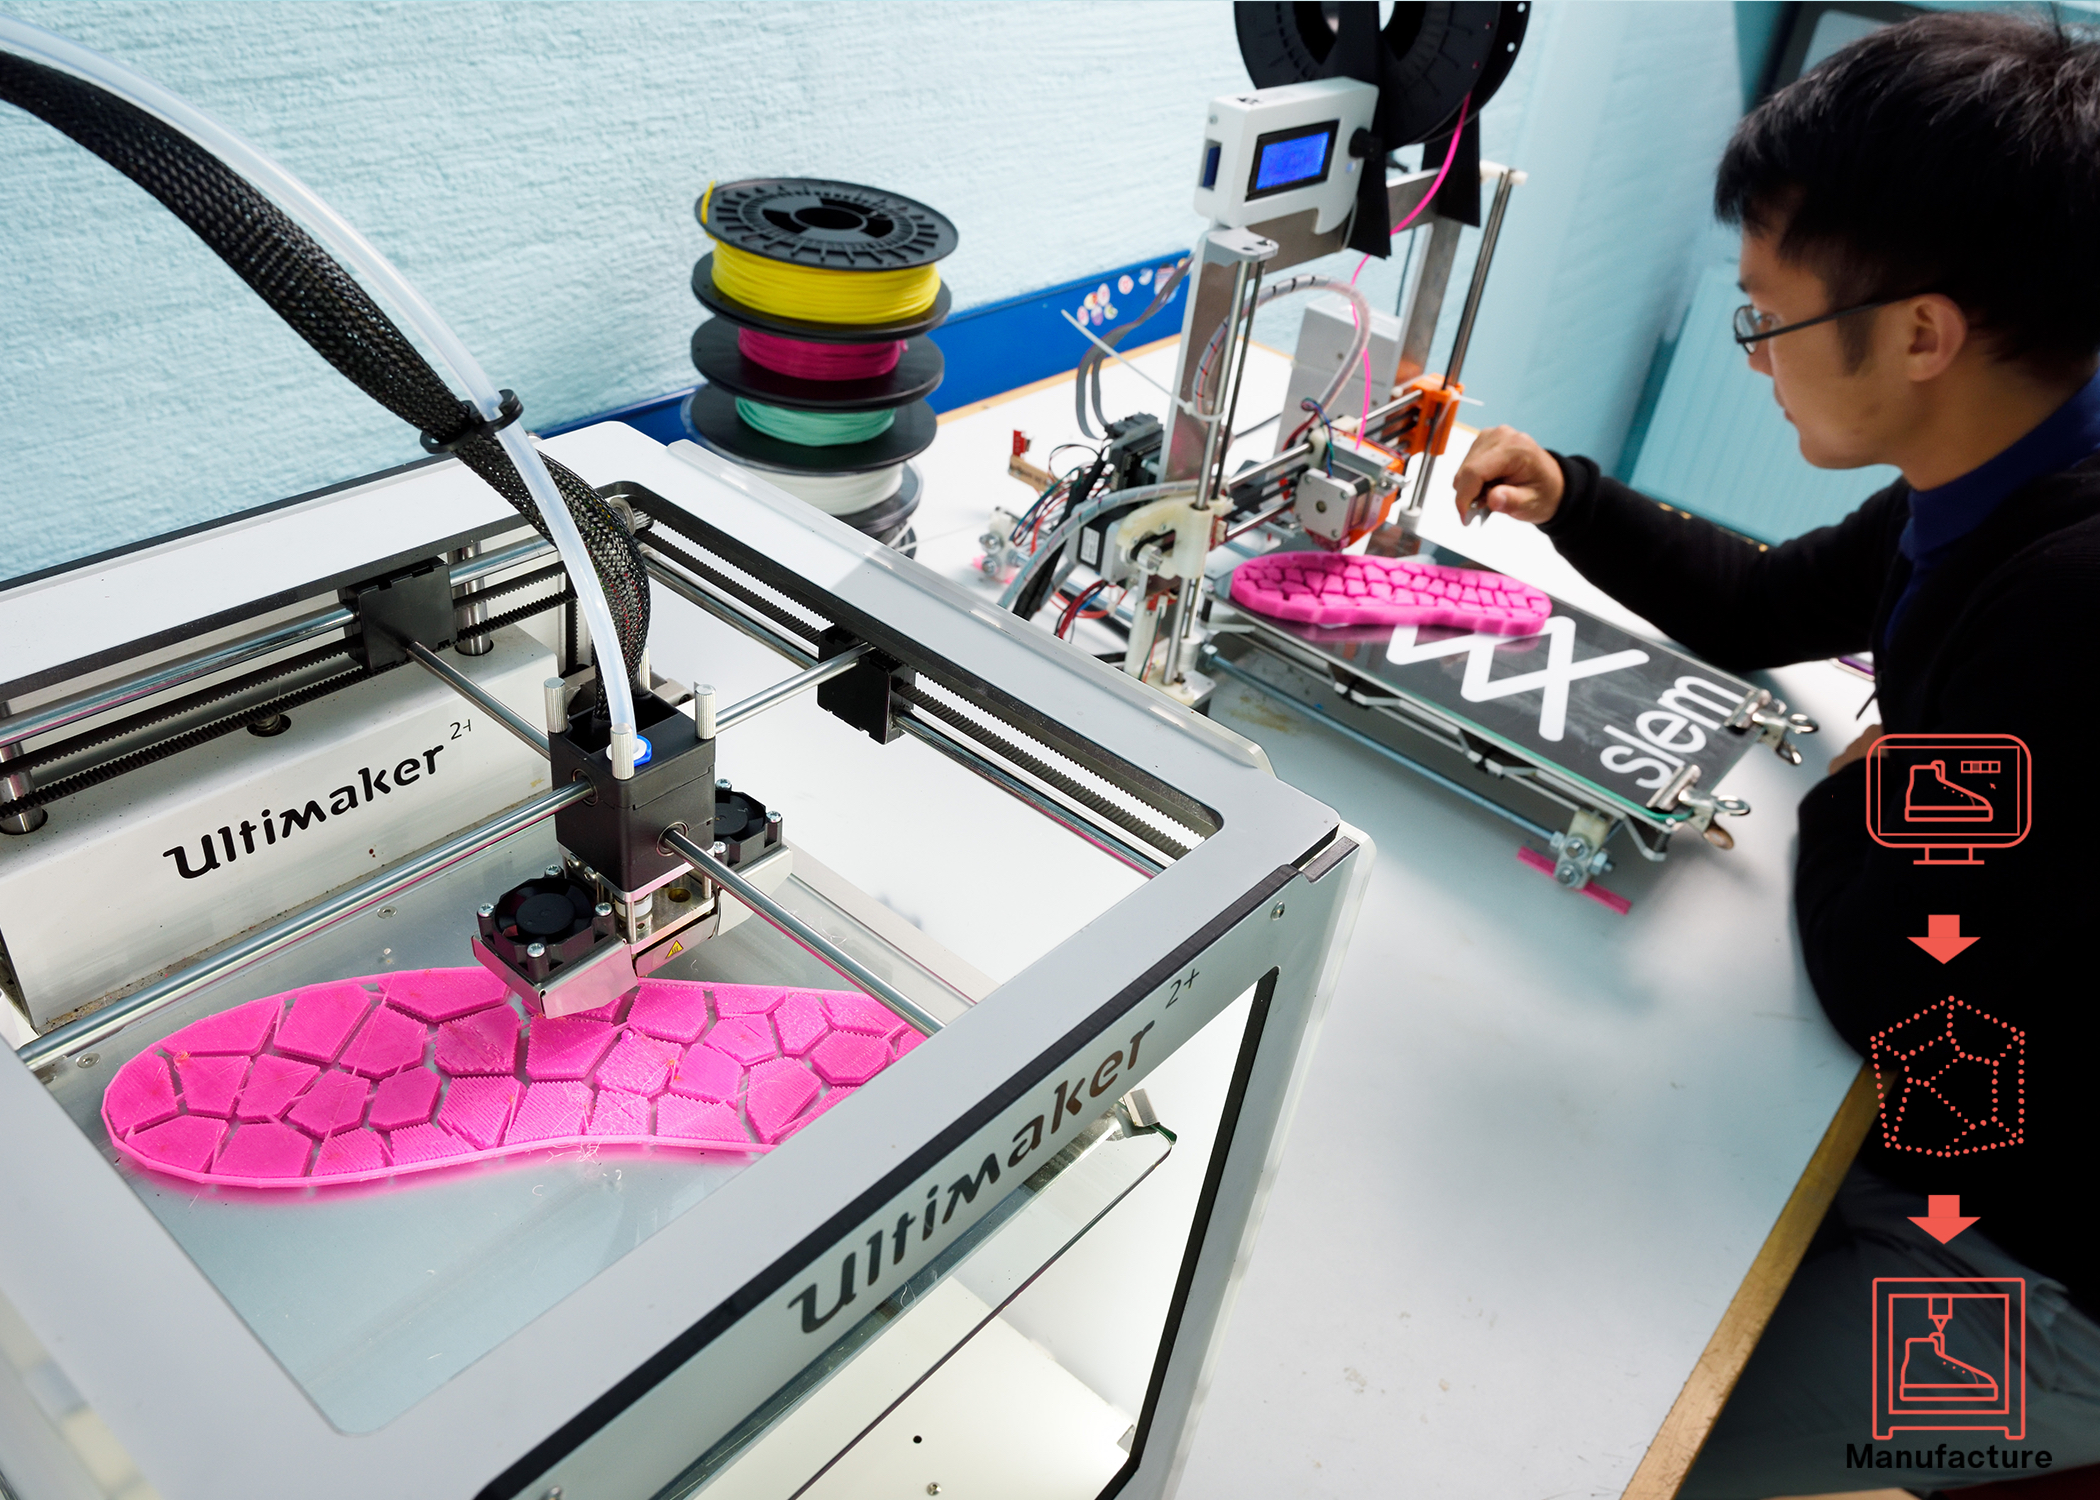
\includegraphics[width=.5\textwidth]{Printing}
\caption{4D pritnting pesonailzed shoe soles using the SoleMaker software and data from project 1. Photo by Bart van Overbeeke}
\label{fig:Project2}
\end{figure}

\subsubsection{Learning 2 Ranges of quality and precision}

We learned the importance of standardizing programmed material behavior. Some areas needed selective buckling \cite{Paulose2015}, such as inside the footbed. Other areas needed rectilinear textile like structures where we could adjust the spacing between rows and columns to create sponge like result, as in the treads of fig. 6. Some regions were very complex and important to the behavior. We found the 3D printer had difficulties with certain structures in certain colors on certain days. We experienced under extrusion leaving areas soft and flimsy, and over extrusion making areas hard and rigid. Having no solution at that moment for  imprecisions in printing, we had to accept to work within ranges of quality in the materials structures. Although, we would later find part of the cause (as described in the next section), this issue also showed us that a hybrid craft requires working with the qualities of the materials available. 

\subsubsection{Challenge 3 Manufacturing misinterpretation}

Once we developed control over the quality and behavior of the tread, footbed, and sidewalls we had another challenge. As explained in learning 2, our standardized programmed material behavior fluctuated over days, and by the filament's color. While negotiating design considerations like the balance and temperature of the shoe, we encountered a problem with the back pressure in the nozzle of the 3D printer. Pressure built up in the nozzle and shifted the programmed extrusion by as much as 8mm when the material exited from the nozzle. Moreover, with certain geometries, not enough material was sometimes deposited creating stringy and sometimes broken filament extrusions. 

Several tricks were invented and taught to us by the 3D printer maker Ultimaker to alleviate these problems, but the final product was not exactly what we programmed. We ran a series material tests using an experimental filament flow sensor. These tests allowed us to see exactly how much material was travelling into the print head and helped us to create a better understanding of how gCode was translated by the machine. We found that certain geometries deposited as little as 72\% of the material the code requested. Software changes helped alleviate some of the problems found in certain geometries. Slowing the speed or combing (retracing) the printed line on important areas allowed the back pressure in the nozzle to refill areas. This was applied after sharp direction changes, especially on curves.

\subsubsection{Learning 3 Limits of the current technology}

There are limits to the technologies and materials we are working with. To design material behavior these limits must be accepted or improved upon. Dourish has shown how ``some data is more important than others'' and used an example of a post script compiler \cite{Dourish2017}. 3D printing technology is far from WYSIWYG (what you see is what you get). The quality of the material structures had a level of precision that was similar to the early days of graphic design. We found that certain geometries were far more critical and required more delicacy (slower speeds and more detail in gCode). To design we not only had to understand the quality and precision, we had to understand where the important areas were and take measures such to increase precision. Iterative personalization required us to adapt our tools and techniques alongside the software in a dynamic way. 

\subsection{Project 3: Encoding a Data Structure}

\begin{figure}
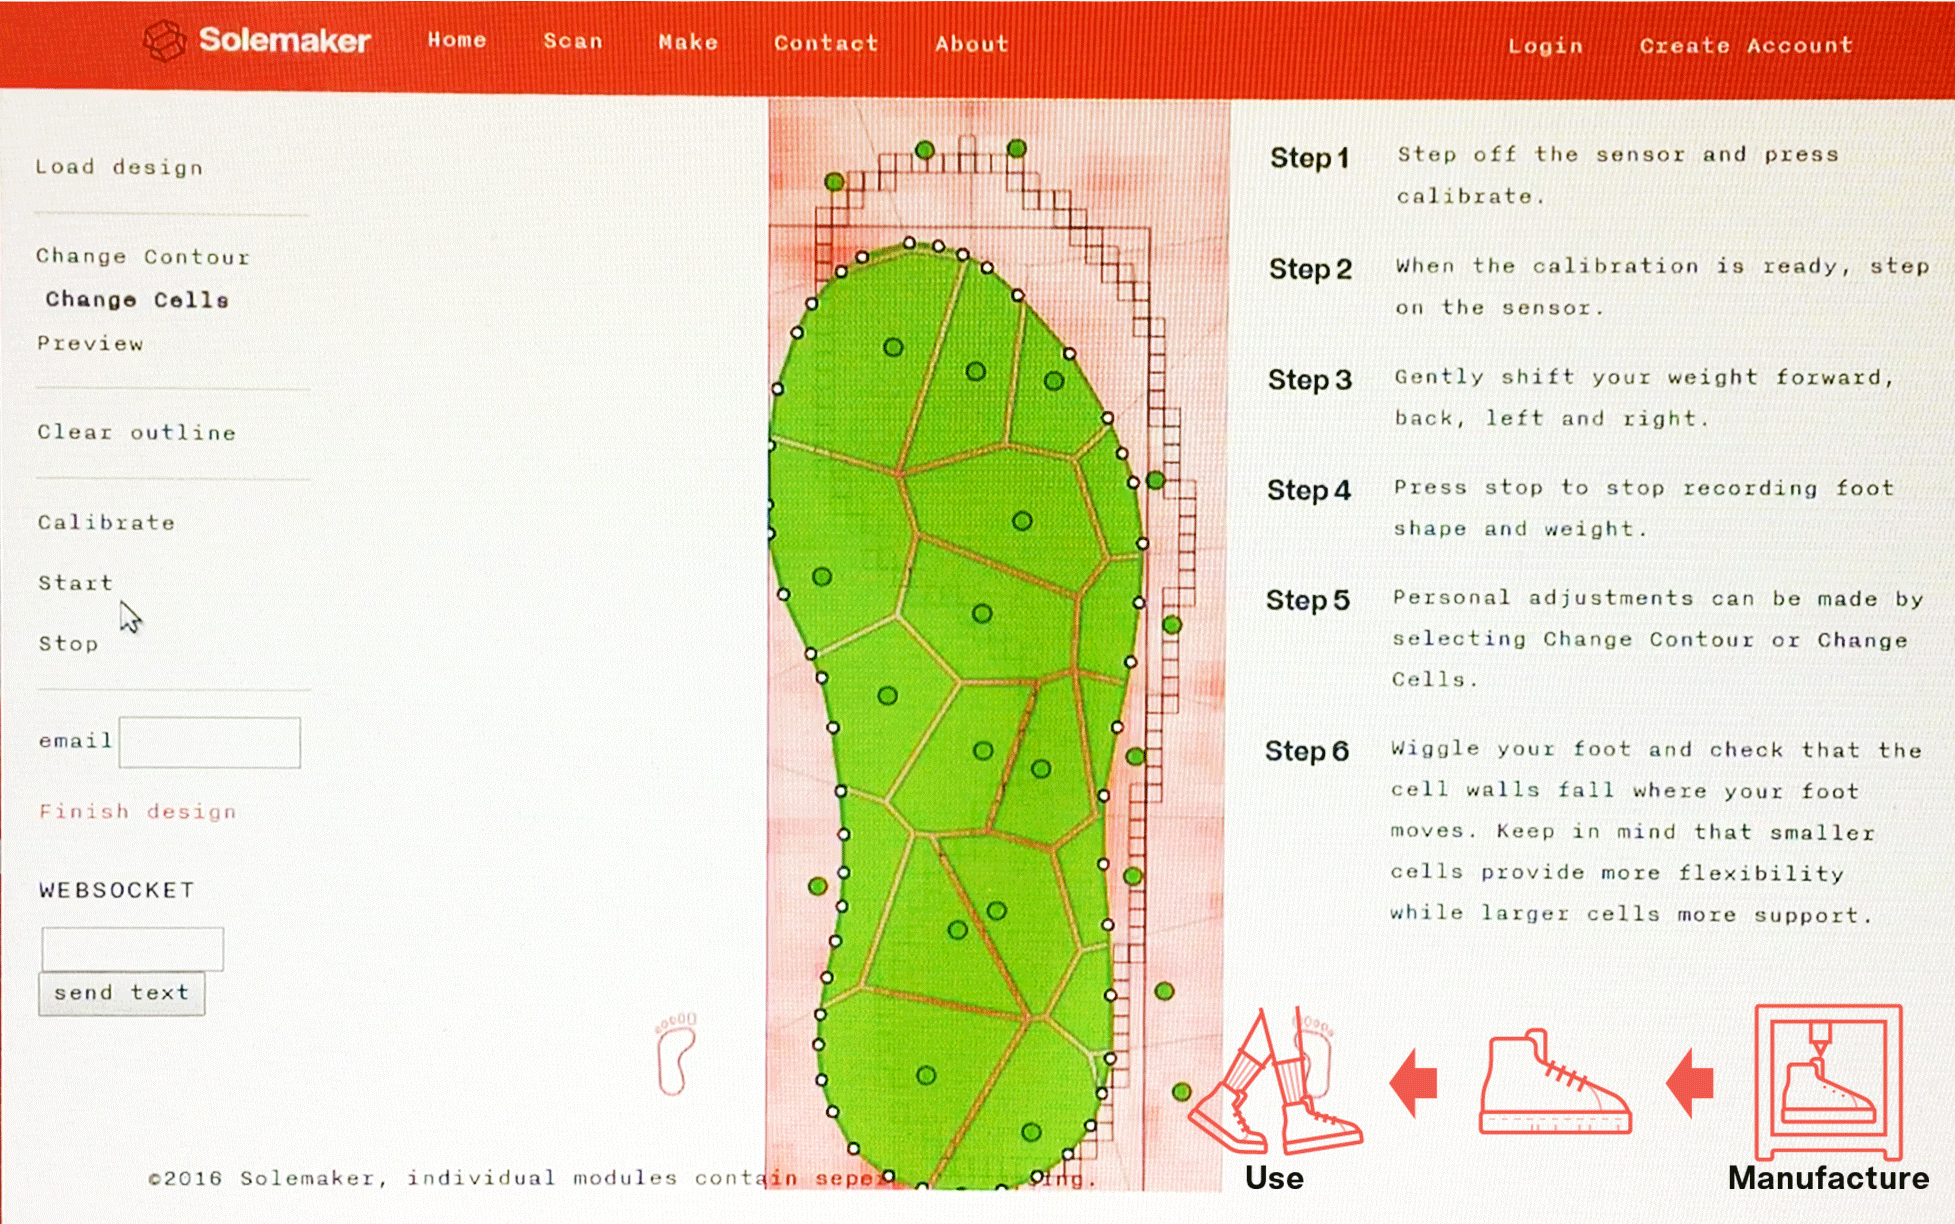
\includegraphics[width=.5\textwidth]{Solemaker_io}
\caption{Screenshot of the web interface of the online version of project 3. Data from project 1 is imposed under the design software from project 2 }
\label{fig:Project3}
\end{figure}

With our understanding of the need for machine learning and with the complexity of the system growing we needed a place to save and store foot scans, temporal composite .json files, design files and digital fabrication files. Iterative personalization required a data trail structure to store that data between iterations. Project 3 was a web platform that created a web interface and a database to profile the shoe analysis, design, manufacture and use. The web platform was built with Docker modules that supported all the other code: the pressure pad scanning software, the sole tread software, and the uppers generator software alongside social log-ins, a QR code generator and database system (see figure 5). 

\subsubsection{Challenge 1 Saving and storing the data trail}

While attaching the pressure pad scanning module data to shoe design software we realized how complex the data gathered to the generate the shoes could be for a single user. Developing the web platform in project 3 taught us how to encode data and store it for multiple iterations and multiple users. The web platform provided a place to save and store the information together enabling the profiling and comparison of data.
This data included: 1) The pressure pad scanning temporal composite as a .json file. 2) The raw stream of data with as much as 100mb per scan. 3) The data from the sole software and the shoe upper generator stored as a .json containing the contour array, and tread Voronoi seed point array. 4) The machine code as  a .gCode file, .svg and instruction manual. 5) A field in the database for the filament flow sensor (for future documenting ranges of quality in material structure). This was connected to a social login module was added to allow users to integrate Facebook, Twitter, LinkedIn, GitHub, QR code or email. 


\subsubsection{Learning 1 Ideal vs actual}

Applying the idea of digital twining is difficult in an everyday context. Digital/physical twins may be born identical, but they grow into unique individuals. As we started to look at profiling and use data, we learned that there was an opportunity to track the differences between the ideal and actual shoe. Storing all this data allowed a quality check from the material production cycle and could be used instead of rigorous physical testing of the manufactured shoe. If we consider that 3D printing implies a distributed co-manufacturing \cite{Nachtigall2019} system of many people with printers in many locations, this type of data becomes vital. The comparison between ideal and actual seemed to be true across multiple iteration of shoes as well. The past data could be used to not only to control and generate the next pair of shoes, but a whole closet of shoes for different users' needs and desires. It was also important to understand the distinction between the ideal designed version and the actual manufactured version of the shoe. The actual version of the shoes is not identical to the ideal version.  

\subsubsection{Challenge 2 Quantity and Scaling up}

The web platform gave us a way to store hundreds and thousands of feet into the system due to its modular construction and scalable architecture. The majority of our modules ran in a browser, saving any risk of the server being overtaxed. This helped us to address concerns around security as well. All data about the foot and generated shoe was stored in the user's browser until it was uploaded to the web platform at the end of the process. Users could log in with their social networks or by email as mentioned in the last section. We also gave them the possibility of generating a QR code that would link to an anonymous account.

\subsubsection{Learning 2 Profiling the thing (shoe), not (only) the person}

There is an opportunity for integrating more data sources resulting in better personalized results. An important learning in project 3 was that we could profile the shoe and not necessarily the person. This allowed a deeper understanding of the material of the shoe. We realized the iterative personalized process was a shoe to shoe process. Conversely, we realized that sociometric and psychometric data on top of our physiometric data could help us make lifestyle predictions for the fashion of the shoe. This made us more acutely aware of how we could use machine learning (as explained in project 1). 

\subsubsection{Challenge 3 Profiling for predicted use}

Simple calculations of the user's weight and the physics of the material lifespan allowed a general prediction of how long the shoe should last. We combined this with a supposition of our shoe designer on to how long the styles we developed would remain in fashion. With this information, we could estimate how long the shoes would last in terms of steps.  However, we also realized that we did not have information on how much we expected the person to wear the shoe (just how long we expected the aesthetics to remain fashionable). These simple simulations hold much potential for just in time manufacturing, sustainability and material lifetime coordination.  

\subsubsection{Learning 3 Potential for self-directed machine learning}

With more than 400 scans in the system, we had enough virtually generated shoes to begin comparing the resulting files. We learned that we could predict use and compare it to the actual use across user populations. While we did not apply it in this research, it is clear from our understanding of the database that machine learning techniques could be applied. These techniques have the potential to enhance the experience of the worn shoe not only in an iterative way, but across entire populations. Moreover, key to iterative personalization was comparing users to themselves over time and seeing how others who are slightly older may also relate. It is clear that machine learning has the potential of becoming a vital tool in this encoding process.

\subsection{Project 4: Encoding Materials that Encode Data}


\begin{figure}
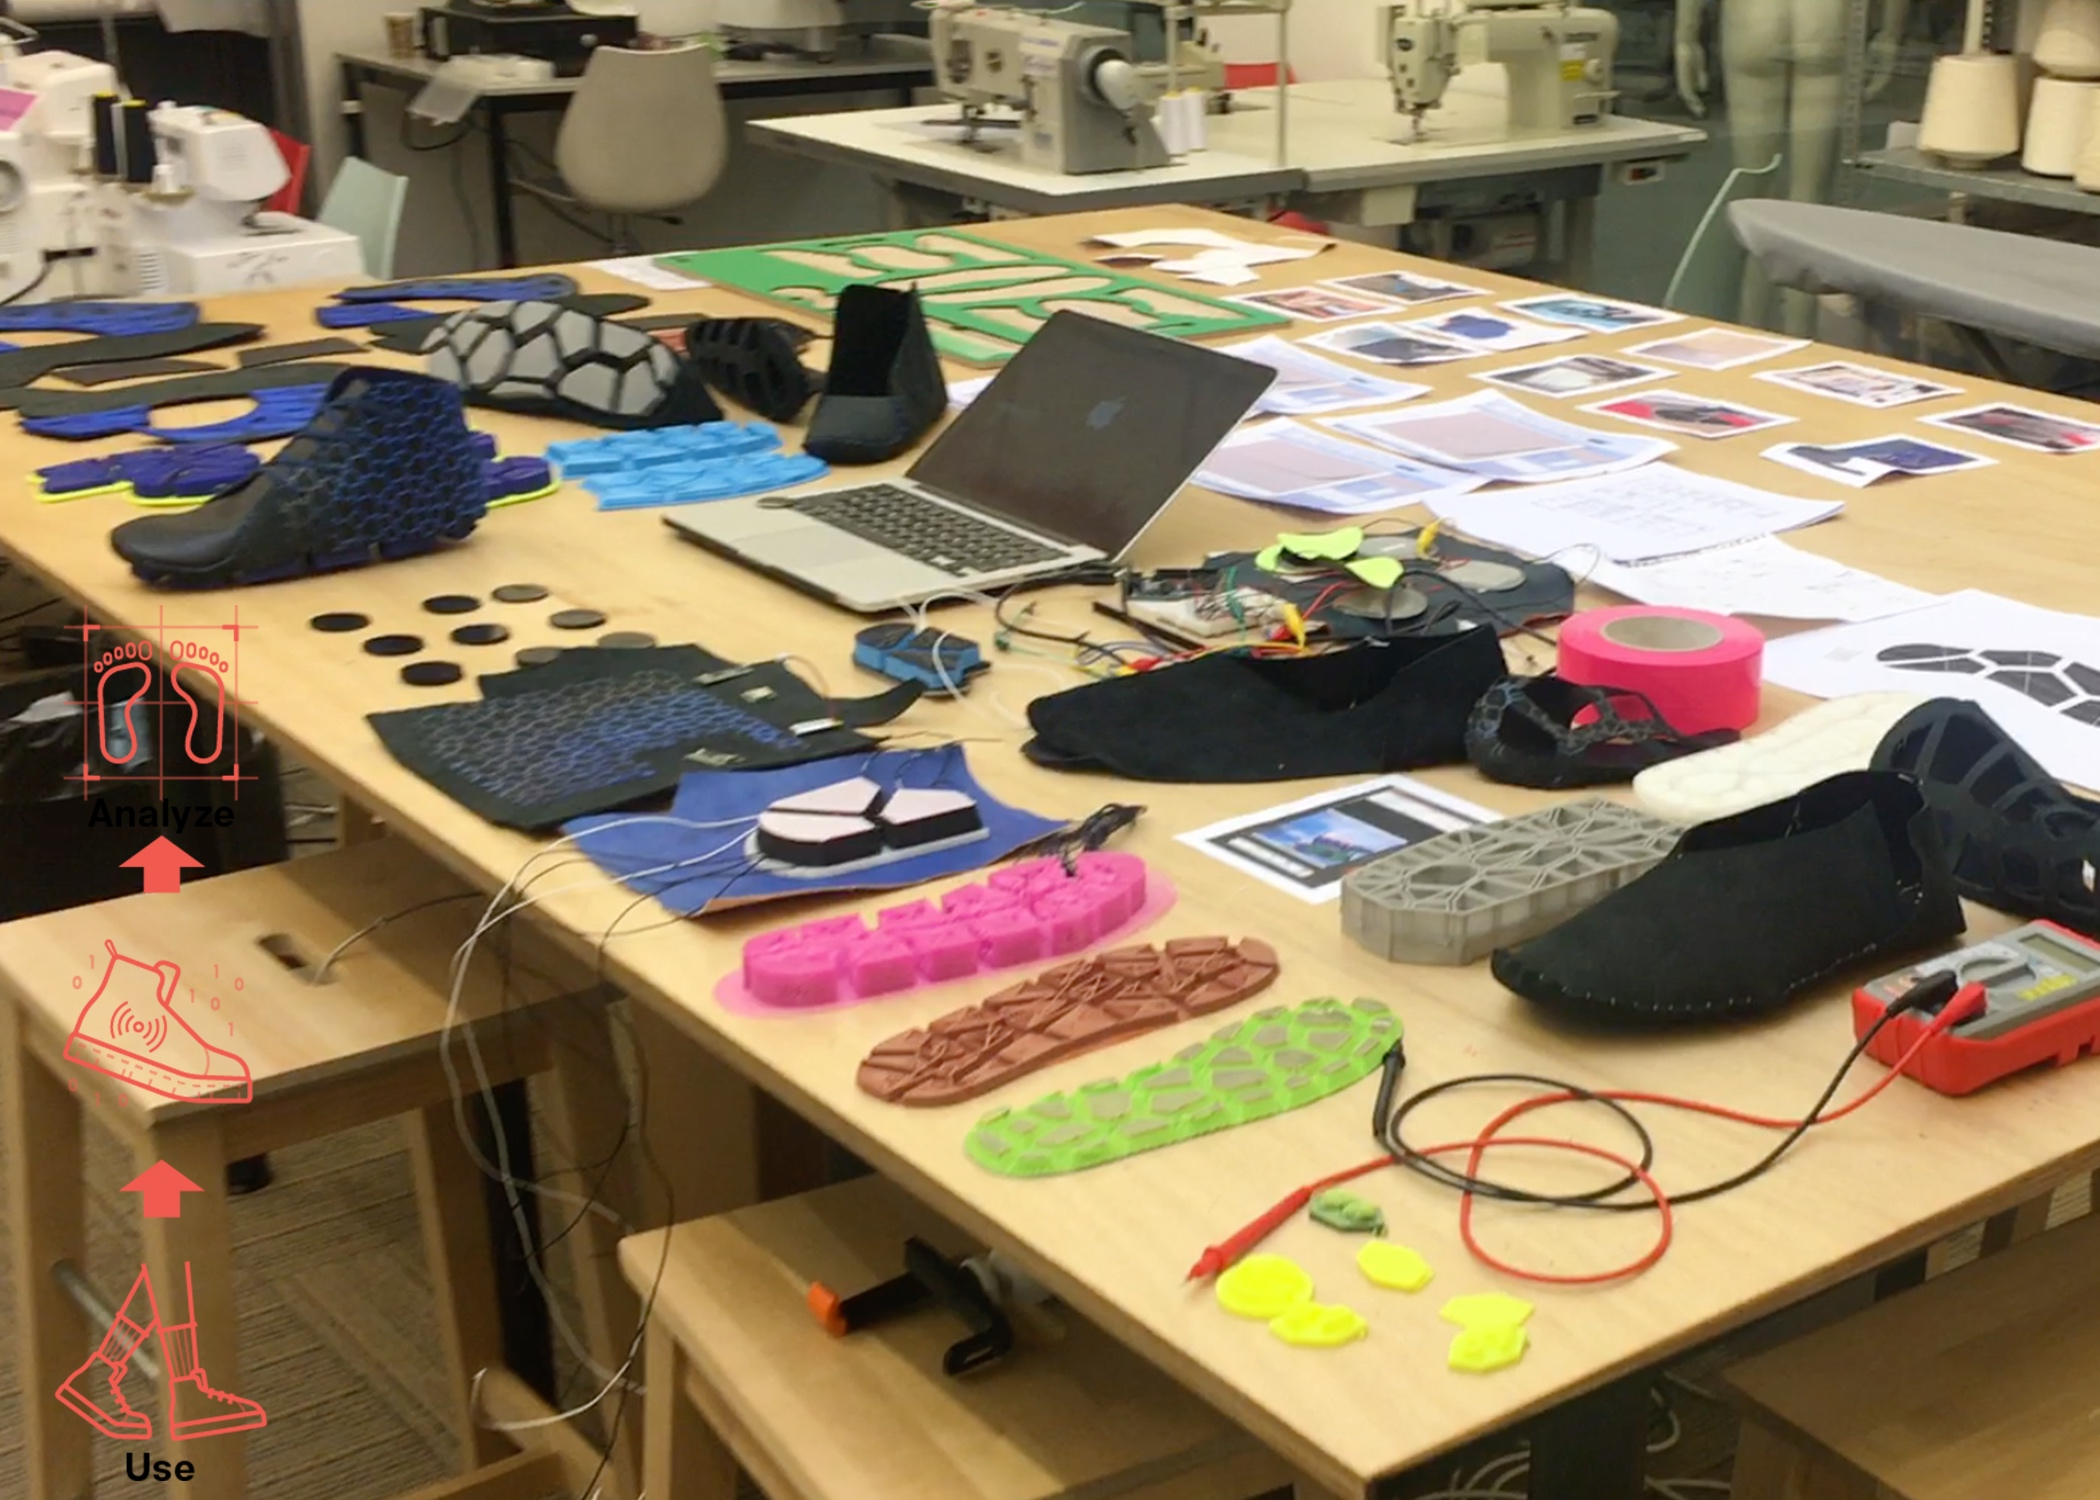
\includegraphics[width=.5\textwidth]{Eva}
\caption{A selection of the several samples developed to create electronic and mechanical sensing inside the structure of the shoe soles.}
\label{fig:Project4}
\end{figure}

Project 3 showed us that we could manage data across the shoe iterations and users, but as seen in project 1, personalization only improves if the sensing of the individual becomes more precise. Our final project looked at encoding data from the shoe while it was in use. We did that by integrating electronics and encoding material structures to store data about the size, pressure and behavior based on criteria established in the first two projects (see figure 6 for an overview the process followed). Previous work by Autodesk into iterative generation of car chassis \cite{Nourbakhsh2016} helped guide our process of generating data in project 4. We worked with a shoe designer to change the style of the shoe to a moccasin construction to solve the problem of sewing the sole to the upper. This change, provided a space for electronics and made it possible to swap the sole. In short, making the project more sustainable and a better research product.

\subsubsection{Challenge 1 Adding electronic sensing to the shoe}

Adding sensing capabilities to a shoe was not easy. We first 3D Printed textile like structures using conductive PI-ETPU 95 filament to create sensors in the sole. Electrodes were manually added to the 3D Printing using small gauge wire in the footbed of the shoe. We created a row/column scanning matrix with a 4 x 10 resolution crossing in points specifically designed to register pressure in the key areas identified in project 1. These were connected to an Arduino Teensy and data was logged at 20hz. The textile structures, previously mentioned, were varied so structures previously designed for comfort, robustness and flexibility would also act as pressure sensors. These sensors were printed for specific force ranges identified from the first scans. For example, the heel sensor was made for a much higher impact force than the four smaller toe sensors.

Changing the filament to conductive ETPU had large impacts on the comfort and flexibility of the shoe. ETPU was far less flexible. We had to renegotiate the design considerations of the footbed to provide comfort to the foot and insulate the electronics. We developed a new triangular textile weave pattern (warp, weft, \& werf) that created a softer material behavior to counter the stiffness of the sensor. It also added more flexibility. 

\subsubsection{Learning 1 Multi-purpose hybrid material geometries}

Creating multi-purpose hybrid geometries that could perform electronic sensing alongside its material properties was a great discovery. However, combining its properties with the design considerations previously encoded in the material was challenging. The new  geometries needed to be significantly different because of the specific material properties of the conductive filaments. Being aware of how to negotiate design considerations (leaning 1 in project 2) made the team ready, and more importantly willing, to deal with the additional complexity required to create the multi-purpose hybrid geometries. Engaging in the hybrid crafting process enabled even greater possibilities as the challenge of adding sensing capabilities became a new design consideration. 


\subsubsection{Challenge 2 Mechanical Sensing Material Structures}

As an additional technique to store the use, we looked at making structures that would break over time, much like winter tire treads. We learned in project 1 that generating a shoe with foot data required making a temporal composite of the footstep. In this project, we explored if we could encode material structures that changed with use to create a mechanical temporal composite. We saw an opportunity to use the material property of breakage with selective buckling \cite{Paulose2015} in the shoe tread. This required maintaining the density control from project 2 and adding small single lines of filament into the buckling structure every four layers. These layers would stretch and eventually break. A small sensing system was developed that would measure if each single line was broken after being used. 

\subsubsection{Learning 2 Active vs passive monitoring}

There are times to use active sensing, and times to use passive sensing. During the testing, we realized it was complicated to read the single line sensors with a 3D printer-based system as there was a deformation of the overall material with wear and tear. While it was possible by hand, it required a lot of time. What we did notice is that in areas of heavy pressure, the shape of the overall geometry of the tread had changed due to the breaking of the internal pieces. First seen as a problem, we rapidly found out inspiration for a way of combining wear and tear, with an evolving form of the shoe sole.

\subsubsection{Challenge 3 Storing and decoding use}

Beyond electronic and material geometry-breaking, we used color change to indicate abrasion. We were inspired by wearing a pair of shoes seen in fig 1. (the third image starting from the left) for many months and noticing abrasion in the material in the talon and heel. For the first twelve layers of material (2.4 mm in height) we added material color changes every four layers. Pictures were taken of the soles in use and using the method of photogrammetry described in \cite{Nachtigall2017} we were able to see how much material had worn off due to abrasion. As this often indicates when someone walked incorrectly, we were able to see where a stronger material would be needed. 

\subsubsection{Learning 3 Understanding temporal composites as material}

We learned that the material itself could store data about use to be decoded later if designed to do so. Each of the three methods told the story of use differently by creating different data trails. Combining all three, they painted a larger picture, but turning the iterative corner required a deep material/data relationship. Based on past experiences 3D printing shoes. we had a preconception that using textile like geometries was superior to selective buckling and meta-materials. We ended up using all three techniques in project 4 to create the encoded material with negotiated design characteristics and sensing/storing capabilities. 

\section{Reflection }
With project 4, we were able to close the iterative personalization loop. The data used in project 4 was more precise than the original data from project 1. In the previous section, we presented our challenges and learnings (see table 1). In this section, we try to summarize them in an effort to make our work transferable to other researchers interested in ultra-personalization. More specifically we discuss encoding material, encoding data and the data/material relationships that developed during the 4 projects.

\subsection{Encoding Materials}
Encoding materials with form, behavior and sensing required creating multi-purpose geometries often with multiple materials. We learned to create these by negotiating design considerations while programming to make 3D printer gCode. This started simply as  density vs. flexibility. It allowed us to approach sensing as if it were just another design considertion of the shoe. This was achieved by many people working together to adapt the generative algorithms while having a deep understanding of the material (ie. flexible filament), tools (ie.3D Printer), techniques (ie. gCode commanding the printer) and data(.json pressure files). It was complex and required people from several disciplines willing to engage in hybrid craft. Creating the encoded material required not only new tools and techniques but also an open attitude and varied skill set.

3D printing flexible materials geometries requires designers to work in ranges of quality and precision when programming the materials structures. We worked through the challenge of standardizing the programmed material behavior accepting that there are ranges of quality that are defined by the Technology (3D Printer), material (the filament, not only the type, but also color) and, as we learned in the process, the direction of travel in creating the geometry itself. Part of the discipline of hybrid crafting is a deep understanding of how digital tools works and how to program them.

Starting off trying to build an electronic sensor shoe would have taken us down a very different journey. We arrived at iterative personalization thanks to the fact that we chose to hybrid craft a bespoke shoe in a full wearable research product. Wearing the shoes while making the shoes inspired us to go deeper. Others have previously integrated off the shelf electronic sensors for iterative improvement, but our work at a base material level allowed us to personalize the sensor itself. It may seem obvious that personalized sensors would create more personalized data, but only by 3D printing electronic sensors we did realize from first-hand experience that we had several opportunities to gather better data. This exploration opened the door to mechanical sensing. 

 Mechanical (non-electronic) wear and tear sensing from encoded structures could be used in many places, not only in shoes, but in many other places where wear and tear is important. We were surprised during our research to discover that some snow tires already use material indicators in the tread. Most interesting from our research was the idea that mechanical sensing could be programmed to already provide a temporal composite for iterative personalization instead of computing one from the electronic sensors. 
 
Designers, makers and researchers often think of 3D printers to be like paper printers. Our experience was the 3D Printer more closely resembles a knitting machine. A knitting machine works with ranges of tensions and yarns. There is a precision to the size of the stitches in a sweater that lends itself to certain kinds of patterns and motifs. There are fundamental rules about how far a single color of yarn can jump before the thread comes loose or how many stitches can be jumped. There is a quality a knitting machine can achieve that we see in material structures essential in both knitting and 3D printing. Our experience in this process was that new insights informing digital fabrication came from people who work with textile machinery. There are limits to the technologies, but experience with tools from other disciplines helps understand those limits in new ways.

\subsection{Encoding Data}

Encoding data for iterative personalization needs compressing time into a temporal composite to provide parameters to the  generative algorithms that encode the material. This temporal composite is in a way an impressionist painting like Picasso's 1938 'Seated Woman' where the painter combines many moments from many painting sessions. We condensed the behavior of users footstep in a computational way of understanding movement over time. This idea of a paining asks more questions such as how do we capture different activities that the wearer is engaged in? Can we encode data that captures enough of a specific behavior that we can understand as designers it is happening?  Do we need to understand or is this a question of precision and interpretation?

Personalizing the sensor to the individual results in better data, but it is not exactly the same format of data. In  encoding data for design, the process used to generate the temporal composite needs to be rewritten. The designers need data to understand how to create temporal composites in a way that creates a better shoe. Unlike current objects that are designed once and mass manufactured, iterative personalization requires the designer to stay involved in the product service system to interpret this data and create new styles. We expect that designers of such system will share our experience that the temporal composite becomes a design material. This is especially true as we consider the difference between the active electronic sensing versus the passive mechanical sensing. 

We see many kinds of quality and precision, not only in the encoded material but also in the encoded data. This includes the data available, the materialization processes, the system training, the negotiated algorithmic generation, and challenges with incorporating new shoes designs into the system. As discussed in encoding materials, the precision of the encoded material is different than the encoded data, we see this as a relationship between the ideal, predicted and actual use. In iterative personalization, we need to be able to compare each iteration so that the level of personalization can grow. The data trail of an object is the narrative story that informs generations to come.  

Iterative personalization requires that the system is trained to be better over each version, just like user statistics improve software in each version. This is an evolutionary system that requires software and algorithms to be trained regularly. The iterative personalization loop is also a feedback loop where we can tell from the data if our data profile of the shoe is correct. Not only can we compare shoes, the encoded data from analysis and profiling is ripe for machine learning. Not only can we compare each shoe version to the previous one. We can compare similar size and pressure patterns over time, and the ideal vs actual shoe that was made to name to name a few. As the database grows with multiple users and multiple shoe versions, it is clear that self-directed machine learning will become a key tool in dealing with the complexity of the data.  

\subsection{The Data/Material Relationship}
In working over two years to encode materials and data for iterative personalization we noted the data \& material relationships changed. In the beginning, the materials we were designing with were the physical filament fed into the 3D Printer. As we came to be familiar with the idiosyncrasies of the material (every color of filament is different, the data from the footscan is a temporal composite), tools (3D printers are susceptible to ambient temperature, humidity, time of day, electric line tension…), and techniques something magic happened. The algorithms used to encode the design characteristics and sensing became really important. The project members began to speak of the algorithms as if they were the material. Not using 3D files, but rather generating gCode and seeing it for the first time on the printer prevented abstraction by a screen. We found ourselves voraciously adding code libraries to control the data just slightly differently. We found our team at the white board rearranging the pressure calculations to make the pressure sensing slightly more sensitive to high impact pressure for someone who is running. Several of these instances changed the design language of the lab we worked in. Hybrid crafting resulted in a new discipline of designing data and material relationships over time. 

The sense of time that iterative personalization changed our role as designer. Depending upon the moment of the lifetime of the shoe we found our activities and perceptions changing. Time is a key element in what we made. The temporal form of the shoe depended upon where we were at in the UPPS cycle. Sometimes the 'shoe' was pure data, some times it was material. Developing the skills to see the shoe as both unlocked the possibilities of iterative personalization. Data allowed us to move through the temporal form of the shoe and capture moments of that lifetime. 

\section{Discussion, Conclusions and Future~Work}
In this paper, we reported on four iterative projects that form a system of iterative personalization. We contribute with lessons learned and techniques for traversing the encoding of data and materials. Our exploratory work aims to enrich the possibilities for makers, designers, engineers and researchers who are developing data-material relationships, especially as a hybrid craft. We extend the capabilities of prior work into material programming \cite{Vallgarda2016} and contribute to the understanding of encoding materials designed with generative algorithms from encoded data. Along the journey, we show new tools and techniques for computational design emerging and a trans-disciplinary understanding of data and materials developing in design. 

Iterative personalization is a making something more personalized by using a data trail created by previous from generations. Iterative personalization might be seen as combining the iterative improvement for design synthesis by Autodesk Research \cite{Nourbakhsh2016} with Vallg\aa rda et al's ideas of temporal design \cite{Vallgarda2015} as iterations over a lifetime.  This opens up a door to not only our sneakers being increasingly personalized every time they become worn out, but that the sneakers encode data for all our shoes including dress shoes, running shoes, high heels and everyday sneakers. we look forward to encoding the data \& materials for such a closet. 

Iterative Personalization shows the potential of Ultra-Personalization. 
This research demonstrates that the Ultra-Personalized Product Service (UPPS) system is beneficial to the design of systems of iterative personalization. This is achieved by encoding data and encoding materials in ways that remember how the thing was made and used. We show how a product service system can support iterative personalization by subdividing the complexity of the lifetime. Moreover, the collection of data across the lifetime of the shoe opens up possibilities for  post-human concerns such as sustainability, not only over the lifetime of a shoe, but in multiple shoe over multiple lifetimes. The ability to use data as a designer provides new frontiers for hybrid craft, allowing designers to consider the why of the object, not just the how. 

Iterative personalization also builds on the idea of the research product\cite{Odom2016}. Not only does each shoe become a research product for successive shoes, there is a potential that thousands of shoes becomes a research product informing all the other shoes that follow, and perhaps more than show. Our everyday things may combine data across large numbers of artifacts informing each other. New potential for hybrid craft emerge as new outliers and expressions emerge from the data, creating new material geometries. The role of the designer becomes more active in the process as the behavior of individuals changes over time. The cycle in some ways resembles software development working with more software developers in hybrid craft may open more possibilities. 

Understanding and designing the data \& material relationship over the lifetime of an object tells us new things about materials, use, and people in their natural setting. 
The insights gained during this research are only a first step into encoded material and data for iterative personalization. We hope to create several more iterations of the shoes for individual wearers and understand the limits of iterative personalization in shoes. We also hope others will join us to explore the data \& material relationship to iteratively personalize of all kinds everyday things.  


\begin{acks}
We would like to thank Loe Feijs, Stephan Wensveen, Admar Schoonen, Bart Pruijmboom, Eva Klabalova, Henry Lin, Erwin Hoogerwoord, Fiore Basile, Nik van Sleeuwen, Rueben Lekkerkerker, Sigridur Helga Hauksdottir, Annaluisa Franco, Koen van Os, Kristina Andersen the members of the TU/e Wearable Senses Lab, the members of the TU/e /dSearch Lab, the members of the UdK Berlin Design Research Lab , the students and staff of The Footwearist, the members of the H2020 ArcInTexETN, and many others for the support, dedication, and long hours committed to these projects. Special thanks to the Dutch Creative Industries Design United for their generous support. This project has received funding from the European Union's Horizon 2020 research and innovation programme under the Marie Sklodowska-Curie grant agreement No. 642328.
\end{acks}
